\title{etrm: Energy Trading and Risk Management in R}

%\title{The \CRANpkg{etrm} Package: Energy Trading Risk Management}
\author{by Anders D. Sleire}

\maketitle

\abstract{
This paper introduces \CRANpkg{etrm}, an R package with tools for trading and financial risk management in energy markets. Contracts for electric power and natural gas differ from most other commodities due to the fact that physical delivery takes place over a time interval, and not at a specific point in time. There is typically strong seasonality, limited storage and transmission capacity and strong correlation between price and required volume. Such characteristics need to be taken into account when pricing contracts and managing financial risk related to energy procurement. Tools for these task are usually bundled into proprietary Energy Trading Risk Management (ETRM) systems delivered by specialized IT vendors. The \CRANpkg{etrm} package offers a transparent solution for building a forward price curve for energy commodities which is consistent with methods widely used in the industry. The user's fundamental market view may be combined with contract price quotes to form a forward curve that replicate current market prices, as described in \citet{ollmar2003analysis} and \citet{benth2007extracting}. \CRANpkg{etrm} also provides implementations of five portfolio insurance trading strategies for energy price risk management. The forward market curve and the energy price hedging strategies are core elements in an ETRM system, which to the best of the author's knowledge has not been previously available in the R ecosystem.
}

\section{Introduction}
The purpose of this paper is to introduce the R package \CRANpkg{etrm} and its tools for energy trading and financial risk management. Substantial fluctuations in energy prices represent a significant risk for market players, in particular for large consumers, producers and utility companies, see \citet{1043596}. The price dynamics is complex due to strong weather dependency and physical constraints related to storage, distribution, and the introduction of new technology. See for example \cite{NICOLOSI20107257} for an analysis of renewable energy production and the negative prices following extreme events in the German power market. Derivatives securities, such as futures contracts, are often used to hedge against the commodity price risk. Specialized Energy Trading and Risk Management (ETRM) systems provide the necessary tools to handle key activities such as position management, valuation and  risk reporting. Several proprietary alternatives exist. The annual \textit{Energy Risk’s Software Survey} in \citet{Tho98w} gives an overview of major providers along with rankings based on industry polls. There, ETRM systems are divided into the operational categories \textit{derivatives software}, \textit{physical trading and operations software} and \textit{front- and middle-office functionality}. Historically, many system providers within this domain have bundled modules into large monolithic architectures serving a variety of purposes, including accounting and regulatory reporting. During the last decade, a general trend within system development has moved towards splitting software into smaller stand-alone components. The \CRANpkg{etrm} package solely focus on financial trading, and may be viewed as a module for front- and middle-office functionality for energy derivatives. The package currently offers transparent tools for two main ETRM activities 1) construction of forward market curves and 2) implementation of trading strategies for price risk management.
%Topics studied include pricing and hedging in the forward market \citet{bessembinder2002equilibrium} and modelling of spot price processes \citet{janczura2013identifying}, see also  \citet{benth2007non}.

After the liberalization of electricity and gas markets started in the 1990s, a rich research literature emerged. Topics studied include pricing and hedging in the forward market and modelling of spot price processes, see for example \citet{bessembinder2002equilibrium}, \citet{janczura2013identifying} and \citet{benth2007non}. Alternative methods for pricing options in power markets can be found in \citet{burger2004spot} and \citet{benth2014pricing}. Textbooks such as \citet{eydeland2002energy}, \citet{benth2008stochastic} and \citet{kirschen2018fundamentals} may be used to gain a more detailed overview of market structure, available instruments, methods for risk management and the related markets for fuel, freight and weather products. In this paper, we will cover some of the theory regarding forward curve modelling from \citet{ollmar2003analysis} and \citet{benth2007extracting}. The theoretical framework for price risk management is gathered from the \textit{portfolio insurance} literature, see \citet{Leland1980WhoSB}, \citet{perold1988dynamic}, \citet{leland1976evolution}. This will be presented in further detail below.

We would like to note that there are some tools available outside the domain of proprietary ETRM software providers. Two examples are the MathWorks case studies \citet{Sundar} and \citet{Deoras}, focusing on risk assessment for gas-fired power plants and electricity load and price forecasting using MATLAB. These topics are however somewhat ad-hoc, and the supplied code cannot be easily incorporated into a generic ETRM system for general use. Similarly within the R ecosystem, there are related tools in the Rmetrics suite of packages, such as \CRANpkg{fOptions} and \CRANpkg{fPortfolio}, but they are not directly applicable. Due to the unique properties of energy markets, standard methods for generating forward curves in interest rate markets cannot be used either. To fill this gap and provide practitioners and researchers with tools dedicated to energy price risk management, we have created \CRANpkg{etrm}. The package is available on CRAN, and may be installed and loaded into the R environment by running the following commands:
% \code{install.packages("etrm")}
\begin{example*}
\code{if(!require(etrm)==TRUE) \{install.packages("etrm")\}}
\code{library(etrm)}
\end{example*}

The rest of the article is organized as follows. First, we give a brief introduction to energy market forward curves and the maximum smoothness forward curve (MSFC) model. We describe the \CRANpkg{etrm} implementation and provide examples of use. Second, a short treatment of energy price risk management with futures contracts is provided, followed by a presentation of five portfolio insurance models. The \CRANpkg{etrm} implementation is described and illustrated with practical examples for energy portfolios with both short and long market exposure. The third part provide an overview of the \CRANpkg{etrm} package structure, available functions and included data sets. Finally, the last section summarizes the paper and provide some suggestions for future work. 


\section{Energy market forward price curves}
The standardised forwards for electricity and gas are contracts for flow delivery. The underlying commodity is not received at a fixed point in time, but over a time interval. In mature markets, participants can trade a variety of products, both over-the-counter (OTC) and on exchanges such as \href{https://www.nasdaq.com/solutions/european-commodities}{Nasdaq Commodities}, \href{https://www.eex.com/en/}{European Energy Exchange} and the \href{https://www.theice.com/index}{Intercontinental Exchange}. Liquidity is often best in the so called front-products, and there is normally higher activity in contracts for next week, month, quarter and year compared to similar products further ahead in time. Shorter period contracts may not even be available on a longer horizon, and seasonal price variation is thus not directly observable in prices far ahead in time. Transacted volume and prices also inhibit quite pronounced seasonality, during the year, week and within a specific day. For this reason, forward contracts are divided into categories based on a \textit{load pattern}. In the \textit{base load} contracts, volume is delivered at a constant rate during the contract period, while \textit{peak load} products are linked to high volume hours, such as Monday to Friday from 8 am to 8 pm. Other, more exotic load patterns exist, but they are less common. Further details can be found in \citet{eydeland2002energy} and \citet{kirschen2018fundamentals}.

The aim of the energy market forward price curve calculation is to create a compact representation of the forward market, at a given point in time. The curve must be able to price the quoted instruments correctly, while accounting for typical energy market characteristics such as seasonality and (possibly overlapping) contracts for flow delivery. The curve is an essential decision making tool with many uses, such as pricing non-standard supply agreements, investment decisions and risk management.

The topic of forward curve fitting has been studied for decades in interest rate markets, see for example \citet{mcculloch1971measuring} and \citet{anderson1996estimating}. These techniques cannot be applied directly to commodities with flow delivery and strong seasonality in prices. There are several alternative approaches to calculating a forward price curve for energy commodities. In \citet{fleten2003constructing}, market data is combined with forecasts generated by a bottom-up model constrained by the bid/ask spread in order to meet the no-arbitrage condition. \citet{borak2008semiparametric} propose a semiparametric factor model for the forward curve dynamics in electricity markets, while  \citet{hildmann2012combined} develop a calculation method by combining parametric estimation and prediction of futures prices under constraints.

In \CRANpkg{etrm}, we have opted for a method that combines a seasonal function with the maximum smoothness-approach from interest rate markets, see \citet{adams1994fitting}. Hence, we follow the approach in \citet{ollmar2003analysis} and \citet{benth2007extracting}. \textit{Base load} contracts are used to calculate a curve with daily granularity. This method has several benefits. It produces a continuous curve which has a closed form solution, it is fast to calculate, flexible and used by many practitioners in the industry. The next section provide a brief overview of the method, followed by a description of the \CRANpkg{etrm} implementation with examples.


\subsection{Maximum smoothness forward curve model}
Consider a market at time $t$ with $m$ forward contracts available for trading. Let the list
\begin{equation*}
S_t=\left\{{(\tau^s_1,\tau^e_1),(\tau^s_2,\tau^e_2),...,(\tau^s_m,\tau^e_m)}\right\}
\end{equation*}
contain the start and end dates for each of these contracts. The time distance between $\tau^s_i$ and $\tau^e_i$ for a contract $i$ in $1, .., m$ cover standardized periods such as \textit{week}, \textit{month}, \textit{quarter} and \textit{year}. Some of these settlement intervals might overlap, and in order to handle this we create a new list of dates $\left\{t_0,t_1,...,t_n\right\}$ to identify each separate sub period, see Figure \ref{fig:timeline}. The new list is made by sorting all dates in $S_t$ in ascending order and removing duplicates.
%In this paper we will consider contracts that deliver the energy at a constant rate over this interval.

% insert time line here
\begin{figure}[ht!]
\centering
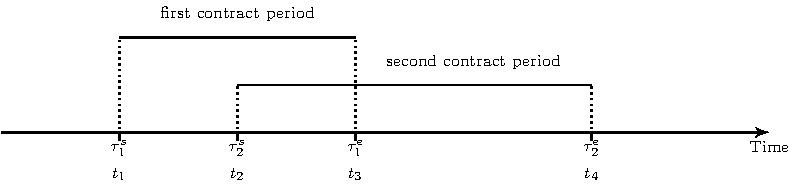
\includegraphics [scale = 1] {timeline.pdf}
\caption{Illustration of two overlapping contracts with start ($\tau^s$) and end ($\tau^e$) dates. Due to the overlap, the total delivery period is split into sub intervals identified with $\left\{t_1,t_2,t_3,t_4\right\}$.}
\label{fig:timeline}
\end{figure}

%When we describe them, we will follow the procedure in \citet{rasmussen2000valuation}.
The forward price at time $t$ for one unit of energy delivered at a constant rate $(\tau^e-\tau^s)^{-1}$ over the time interval $(\tau^s,\tau^e)$ is denoted by $F(t,\tau^s,\tau^e)$, where $t\leq\tau^s<\tau^e$.  A forward contract for a flow delivery may be thought of as the average of hypothetical single-delivery contracts. At time t, each of these would have a unique price $f(t,u)$ for the delivery at u with an infinitesimal delivery period. This leads to $F(t,\tau^s,\tau^e)$ being the weighted average 
\begin{equation}
F(t,\tau_s,\tau_e)=\int\limits_{\tau^s}^{\tau^e}{w(u, \tau_s, \tau_e) f(t,u)}\,\mathrm{d}u
\label{fwdprice}
\end{equation}
where $w(u, \tau_s, \tau_e) = \frac{\hat{w}(u)}{\int_{\tau_s}^{\tau_e}\hat{w}(v) dv}$ is a weight function accounting for the rate of interest $r$ and the time value of money. If the contract in question is settled at the end of the delivery period (forward contract), the weight function is given by $w(u, \tau_s, \tau_e) = 1/(\tau_e-\tau_s)$. If the contract is settled continuously over the delivery period (futures contract), $w(u, \tau_s, \tau_e) = \frac{re^{-ru}}{e^{-r\tau_s}-e^{-r\tau_e}}$.  In the following we construct a forward market price curve for the entire horizon using a simplified notation $f(u)$ for the function describing the forward curve at time t. In order to model the strong seasonality in energy markets, the forward curve function is decomposed into two elements:

\begin{equation}
f(u)=\Lambda(u) + \epsilon(u) \qquad {u \in [t_0,t_n] }
\end{equation}

Following \citet{ollmar2003analysis} we calculate $f(u)$ by combining a prior function $\Lambda(u)$ which contain our subjective views on the future prices with an adjustment function $\epsilon(u)$ to ensure match with the observed closing prices for the $m$ contracts. The prior could be generated with a simple sinusoidal function or from a fundamental model more capable of describing the seasonality and calendar effects observed in energy markets. Should the prior be excluded, the seasonal price patterns will not be visible in the far end of the curve, where only yearly or seasonal contracts are available. Smoothing is calculated on the adjustment function, we aim to minimize the total curvature of $\Lambda(u)$ while preserving the information from the prior. Smoothness is defined as the integral of the second-order derivative of the function, and the smoothest possible curve over $[t_0,t_n]$ is achieved by minimising
\begin{equation*}
\int\limits_{t_0}^{t_n}{[\epsilon''(u)]^2}\,\mathrm{d}u
\end{equation*}
under five constraints presented below. \citet{lim2002computing} show the smoothest possible curve is found when the n sub periods are modelled by fourth-degree polynomials. We write $\epsilon(u)$ as a spline
\begin{equation*}
  \epsilon(u)=\begin{cases}
    a_1u^4+b_1u^3+c_1u^2+d_1u+e_1, & {u \in [t_0,t_1] },\\
    a_2u^4+b_2u^3+c_2u^2+d_2u+e_2, & {u \in [t_1,t_2] },\\
      \indent.\\
    	\indent.\\
    a_nu^4+b_nu^3+c_nu^2+d_nu+e_n, & {u \in [t_{n-1},t_n] }.\\
  \end{cases}
\end{equation*}
\\
In order to construct the forward curve function we need to identify the parameters of $\epsilon(u)$
\begin{equation*}
\mathbf{x}^\intercal = [a_1\ b_1\ c_1\ d_1\ e_1\quad a_2\ b_2\ c_2\ d_2\ e_2\dots\
a_n\ b_n\ c_n\ d_n\ e_n]
\end{equation*}
\\
by solving the quadratic optimisation problem

\begin{equation}
\min_{x}{\int\limits_{\tau^s}^{\tau^e}{[\epsilon''(u;x)]^2}\,\mathrm{d}u}\ \label{quadmin}
\end{equation}

\noindent subject to

\begin{align}
(a_{j+1}-a_{j})u_j^4+(b_{j+1}-b_{j})u_j^3+(c_{j+1}-c_{j})u_j^2+(d_{j+1}-d_{j})u_j+e_{j+1}-e_j & = & 0 \label{knotcont} \tag{a} \\
4(a_{j+1}-a_{j})u_j^3+3(b_{j+1}-b_{j})u_j^2+2(c_{j+1}-c_{j})u_j+(d_{j+1}-d_{j}) & = & 0  \label{diffknotcont} \tag{b} \\
12(a_{j+1}-a_{j})u_j^2+6(b_{j+1}-b_{j})u_j+2(c_{j+1}-c_{j}) & = & 0 \label{diff2knotcont} \tag{c}\\
\epsilon'(u_n;x) & = & 0 \label{horizontal} \tag{d} \\
\frac{1}{\tau^e_i-\tau^s_i}\int\limits_{\tau^s_i}^{\tau^e_i}{(\Lambda(u)+\epsilon(u))}\,\mathrm{d}u & = & F^c_i \label{closing} \tag{e}
\end{align}



\noindent for spline knot $j = 1, ..., n-1$ and contract $i = 1, ..., m$. The constraint in \eqref{knotcont} ensures the adjustment function is continuous in the knots, while \eqref{diffknotcont} and \eqref{diff2knotcont} imposes this restriction also for the first and second order differentials. The \eqref{horizontal} constraint require the adjustment function to be horizontal at time $T$, and finally \eqref{closing} also require the average value of the forward price function $f(u)$ over the delivery period for contract $i$ to match the quoted closing price $F^c_i$. Here, we could take the interest rate effect from $r$ into account and set the present value of the average of the forward price function equal to present value of the forward contract. Instead of doing that, we will follow \citet{benth2008stochastic} and \citet{ollmar2003analysis} and assume $r=0$ such that the weight function in \ref{fwdprice} is approximated with $w(u,\tau^s,\tau^e)\approx\frac{1}{\tau^e-\tau^s}$. Like \citet{benth2008stochastic} we will argue that both the prior and the smoothing will outweigh a marginal interest rate effect. This minimisation problem can be expressed as

\begin{equation*}
\min_{\mathbf{x}} \quad {\mathbf{x}^\intercal \mathbf{Hx}},
\end{equation*}
where $\textbf{x}$ is a $(5n \times 1)$ vector and

\begin{equation*}
\textbf{H} =
 \begin{bmatrix}
  h_1 & & 0 \\
  & \ddots & \\
  0 &  & h_n
 \end{bmatrix},
\textbf{h}_j =
 \begin{bmatrix}
  \frac{144}{5}\Delta^5_j & 18\Delta^4_j & 8\Delta^3_j & 0 & 0 \\
  18\Delta^4_j & 12\Delta^3_j & 6\Delta^2_j & 0 & 0 \\
  8\Delta^3_j & 6\Delta^2_j & 4\Delta_j & 0 & 0 \\
  0 & 0 & 0 & 0 & 0\\
  0 & 0 & 0 & 0 & 0\\
 \end{bmatrix}
\end{equation*}
The block diagonal matrix $\textbf{H}$ has dimensions $(5n\times5n)$ and $\Delta_j = t^l_{j+1}-t^l_{j}$. As the constraints in \eqref{quadmin} are all linear in $x$ and may be expressed on the form $\boldsymbol{Ax}=\boldsymbol{B}$, the problem may be rephrased as an unconstrained minimisation problem via the Lagrange multiplier method:

\begin{equation*}
\min_{\mathbf{x},\boldsymbol{\lambda}}  \quad  \boldsymbol{x^\intercal Hx + \lambda^\intercal(Ax-B)}
\end{equation*}

\noindent where $\mathbf{A}$ is a $(3n+m -2 \times 5n)$ matrix and $\mathbf{B}$ is a $(3n+m-2 \times 1)$ vector. The spline parameter vector and Lagrange multipliers are identified by solving

\begin{equation}
 \begin{bmatrix}
  \mathbf{2H} & \mathbf{A^\intercal} \\
  \mathbf{A}  & \mathbf{0}
 \end{bmatrix}
  \begin{bmatrix}
  \mathbf{x} \\
  \boldsymbol{\lambda}
 \end{bmatrix}
 =
 \begin{bmatrix}
  \mathbf{0} \\
  \mathbf{B}  
 \end{bmatrix}
\end{equation}

\noindent where the left matrix has dimension of $(8n+m-2) \times (8n+m-2)$ and both vectors are of dimension $(8n+m-2)$. %Tools for performing this optimisation and calculating the forward curve are described in further detail below.

\subsection{The "MSFC" class with examples}
The forward curve calculation in \CRANpkg{etrm} is implemented in the S4 \code{"MSFC"} class. By supplying all required arguments to the constructor function \code{msfc()}, the user may create an object that contains the calculation results, input arguments and further calculation details. In addition to the arguments from the list of contracts, the user may also provide a prior to the calculation. By default the prior is set to zero, but the user can input any vector expressing a belief regarding the market to be combined with the observed prices. An overview of the \code{msfc()} arguments can be found in Table \ref{msfc_function}.  

\begin{table}[h!]
\centering
\resizebox{10cm}{!}{%
\begin{tabular}{lll}
\toprule
\textbf{Argument} & \textbf{Description} & \textbf{Default value} \\
\midrule
\code{tdate} & Trading date & none \\
\code{include} & Logical vector for contract selection & none \\
\code{contract}  & Character vector with contract names & none \\
\code{sdate}  & Date vector with contract start dates  & none \\
\code{edate} & Date vector with contract end dates & none \\
\code{f} & Numeric vector with contract prices & none \\
\code{prior} & Numeric prior curve vector & 0 \\
\bottomrule
\end{tabular}
}
\caption{Arguments for the \code{msfc()} constructor function for forward curve calculation.}
\label{msfc_function}
\end{table}

The \code{"MSFC"} class properties and available methods are summarised in Figure \ref{fig:msfc_class}, and a brief description is provided in the following. The \code{"Name"} slot describe the type of forward curve model used by storing the character value "MSFC", while \code{"TradeDate"} keeps the trade date used in the calculation. A data frame containing details for selected contracts along with the calculated forward price based on the curve can be found in \code{"BenchSheet"}. A count of the $(n-1)$ number of polynomials used in the spline is available as a scalar value in \code{"Polynomials"}, and the prior curve vector in \code{"PriorFunc"}. The main calculation result is stored in a data frame which contains daily values for all selected contracts along with the calculated forward curve. The data frame span the date range from \code{"TradeDate"} to the end date of the contract furthest ahead in time, and can be found in \code{"Results"}. The interested user may also extract additional information regarding the spline itself. Coefficients for all polynomials can be found in the \code{"SplineCoef"} list and the knotpoints separating them in the numeric vector \code{"KnotPoints"}. Further details regarding the calculation of the daily forward curve values are available in the \code{"CalcDat"} data frame. This table is essentially an extended version of \code{"Results"}, where numeric time vectors and the spline coefficients have been added.

\begin{figure}[h!]
\centering
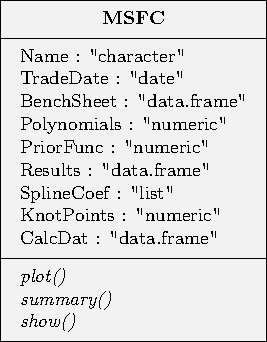
\includegraphics [scale = 0.9] {msfc_class.pdf}
\caption{Attributes and methods of the \code{"MSFC"} class.}
\label{fig:msfc_class}
\end{figure}

The \code{"MSFC"} class has the generic methods \code{plot()}, \code{summary()} and \code{show()}. The \code{plot()} method may be used to create a chart of the calculated curve and underlying contracts from the \code{"Results"} data frame. All plot methods in \CRANpkg{etrm} are based on \CRANpkg{ggplot2}, see \citet{wickham2011ggplot2}. The \code{summary()} method returns a list with three elements; a description string, a sample of the prior vector, and the bench sheet. Finally, the \code{show()} method returns the \code{"Results"} data frame. 

We proceed with a practical example using two of the embedded \CRANpkg{etrm} data sets to represent information available to a European power market participant.  All market-related inputs to the \code{msfc()} constructor (trade date and contract properties) are required arguments. These are collected from a synthetic data set for the trading date 2013-05-13, and can be found in \code{"powfutures130513"} presented in Table \ref{powfutures130513}. Contracts covering long time spans are excluded with \code{include = FALSE} if futures of shorter duration are available for the same time interval in order to preserve the seasonality available in market prices. We use a seasonal prior with high energy prices during the winter season, followed by a drop toward the lower summer levels. It also take into account some well known calendar effects,  such as weekends. The prior is simple, and merely used for illustrative purposes. It can be found in the data set \code{"powpriors130513"} included in the package. A calculation excluding the prior is also added for comparison.

\begin{table}[h!] 
\centering 
\resizebox{9cm}{!}{%
\begin{tabular}{@{\extracolsep{5pt}} cccccc} 
\toprule
\textbf{Include} & \textbf{Contract} & \textbf{Start} & \textbf{End} & \textbf{Closing} \\ 
\midrule
TRUE & W21-13 & 2013-05-20 & 2013-05-26 & $33.65$ \\ 
TRUE & W22-13 & 2013-05-27 & 2013-06-02 & $35.77$ \\ 
TRUE & W23-13 & 2013-06-03 & 2013-06-09 & $36.58$ \\ 
TRUE & W24-13 & 2013-06-10 & 2013-06-16 & $35.93$ \\ 
TRUE & W25-13 & 2013-06-17 & 2013-06-23 & $33.14$ \\ 
TRUE & W26-13 & 2013-06-24 & 2013-06-30 & $34.16$ \\ 
FALSE & MJUN-13 & 2013-06-01 & 2013-06-30 & $35.35$ \\ 
TRUE & MJUL-13 & 2013-07-01 & 2013-07-31 & $33.14$ \\ 
TRUE & MAUG-13 & 2013-08-01 & 2013-08-31 & $35.72$ \\ 
TRUE & MSEP-13 & 2013-09-01 & 2013-09-30 & $38.41$ \\ 
TRUE & MOCT-13 & 2013-10-01 & 2013-10-31 & $38.81$ \\ 
TRUE & MNOV-13 & 2013-11-01 & 2013-11-30 & $40.94$ \\ 
FALSE & Q3-13 & 2013-07-01 & 2013-09-30 & $35.72$ \\ 
TRUE & Q4-13 & 2013-10-01 & 2013-12-31 & $40.53$ \\ 
TRUE & Q1-14 & 2014-01-01 & 2014-03-31 & $42.40$ \\ 
TRUE & Q2-14 & 2014-04-01 & 2014-06-30 & $33.39$ \\ 
TRUE & Q3-14 & 2014-07-01 & 2014-09-30 & $31.78$ \\ 
TRUE & Q4-14 & 2014-10-01 & 2014-12-31 & $38.25$ \\ 
TRUE & Q1-15 & 2015-01-01 & 2015-03-31 & $40.73$ \\ 
TRUE & Q2-15 & 2015-04-01 & 2015-06-30 & $32.64$ \\ 
TRUE & Q3-15 & 2015-07-01 & 2015-09-30 & $30.87$ \\ 
TRUE & Q4-15 & 2015-10-01 & 2015-12-31 & $37.22$ \\ 
FALSE & CAL-14 & 2014-01-01 & 2014-12-31 & $36.43$ \\ 
FALSE & CAL-15 & 2015-01-01 & 2015-12-31 & $35.12$ \\ 
TRUE & CAL-16 & 2016-01-01 & 2016-12-31 & $34.10$ \\ 
FALSE & CAL-17 & 2017-01-01 & 2017-12-31 & $35.22$ \\ 
FALSE & CAL-18 & 2018-01-01 & 2018-12-31 & $36.36$ \\ 
\bottomrule
\end{tabular} 
}
\caption{Closing prices for futures contracts used in the forward curve calculation for 2013-05-13. Contracts are selected for the calculations with the \code{include} vector. Prices for these contracts can be found as horizontal lines in Figure \ref{fig:msfc_fut_wpri}} 
\label{powfutures130513}
\end{table} 


As shown in Figure \ref{fig:msfc_fut_wpri}, the shorter contracts close in time to the trading date clearly reflect a seasonal pattern. This is typical in power markets, where weather and calendar effects have strong influence on transacted volume and price formation. On a longer horizon however, this information is not observable in market prices, as the quoted contracts cover longer time spans. This is where price data may be supplemented with prior knowledge in order to create a representation of the market consistent with both the underlying fundamentals and the listed contracts. The following code will create the \code{"MSFC"} objects and plot calculation results:

\begin{example*}
library(etrm)
library(gridExtra)
data(powfutures130513)
data(powpriors130513)

# instance of MSFC class with prior
fwd.fut.wpri <- msfc(tdate = as.Date("2013-05-13"),
                     include = powfutures130513\$Include,
                     contract = powfutures130513\$Contract,
                     sdate = powfutures130513\$Start,
                     edate = powfutures130513\$End,
                     f = powfutures130513\$Closing,
                     prior = powpriors130513\$mod.prior)

# instance of MSFC class without prior
fwd.fut.npri <- msfc(tdate = as.Date("2013-05-13"),
                     include = powfutures130513\$Include,
                     contract = powfutures130513\$Contract,
                     sdate = powfutures130513\$Start,
                     edate = powfutures130513\$End,
                     f = powfutures130513\$Closing,
                     prior = 0)
                     
                     
                     
                     
                     
                     
                     
# the generic plot() method
pw <- plot(fwd.fut.wpri, ylab = "EUR/MWh", legend = "")
pn <- plot(fwd.fut.npri, ylab = "EUR/MWh", legend = "")

# combine plots
gridExtra::grid.arrange(pw, pn)
\end{example*}


\begin{figure}[hbtp] %[ht!]
\centering
%\vspace{2cm}
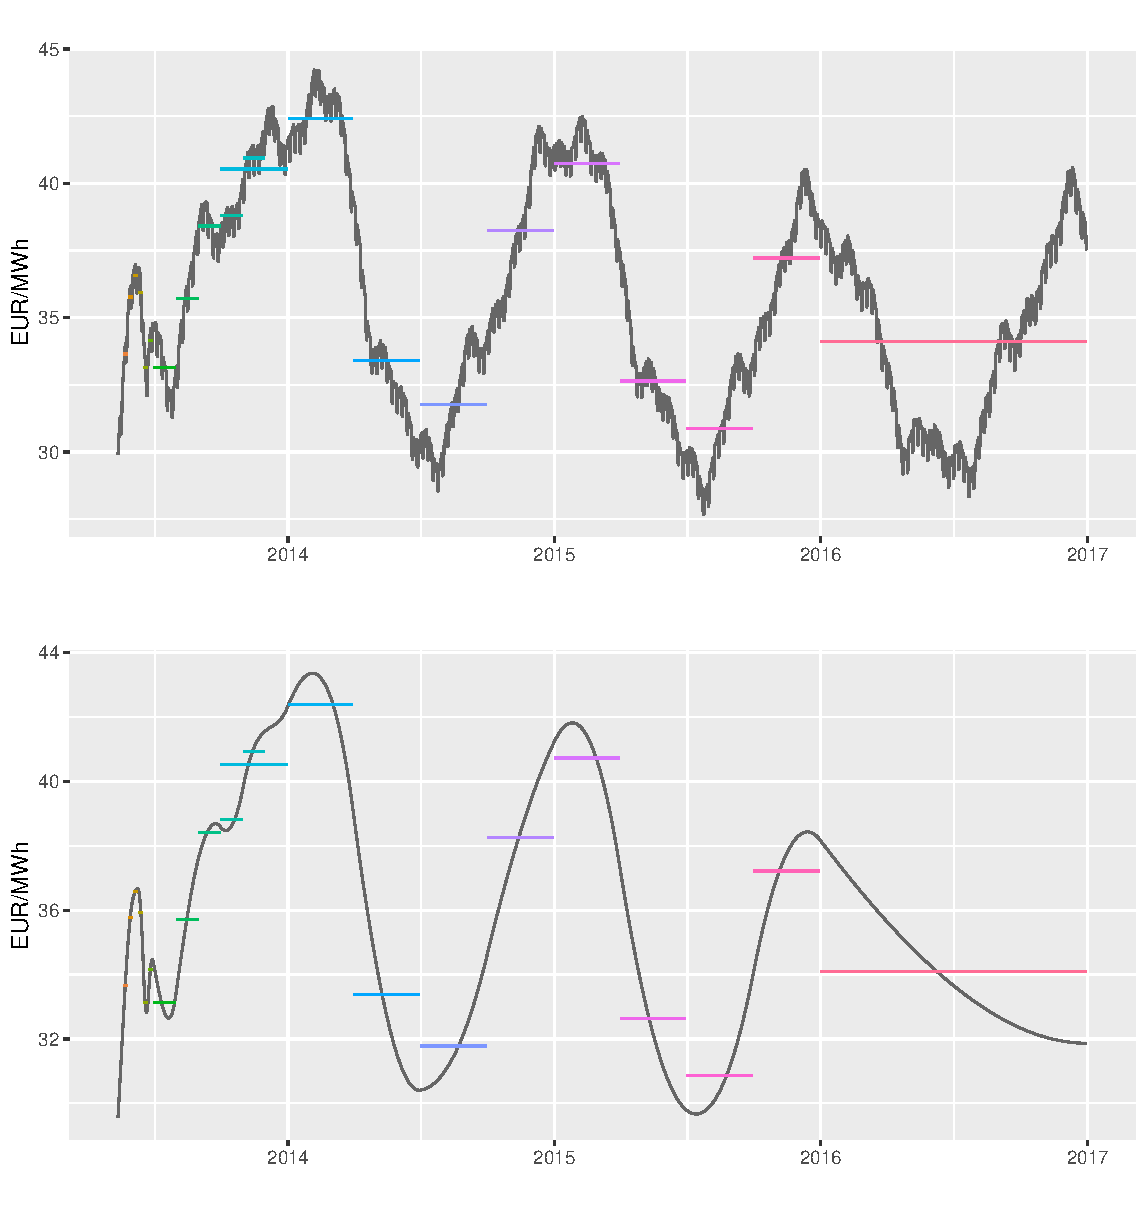
\includegraphics [scale = 0.7] {msfc_fut_port.pdf}
\caption{Two alternative forward curve calculations based on the same contract selection. In the top panel, a prior function is included in the calculation. This curve shows price variation on the weekly level, with lower prices during weekends. The prior also ensures that yearly seasonality is visible in the far end of the curve. The bottom plot is based solely on market prices, which does not reflect seasonality on such long horizon.}
\label{fig:msfc_fut_wpri}
\end{figure}



The computed prices may be verified via the \code{summary()} method, which also return a sample of the prior and information regarding the spline calculation:


\begin{example*}
> summary(fwd.fut.wpri)
\$Description
[1] "MSFC of length 1329 built with 41 polynomials at trade date 2013-05-13"

\$PriorFunc
[1] 30.10842 30.16396 30.19572 30.16144 29.06268 28.93272

\vspace{2cm}

\$BenchSheet
   Include Contract       From         To Price  Comp
1     TRUE   W21-13 2013-05-20 2013-05-26 33.65 33.65
2     TRUE   W22-13 2013-05-27 2013-06-02 35.77 35.77
3     TRUE   W23-13 2013-06-03 2013-06-09 36.58 36.58
4     TRUE   W24-13 2013-06-10 2013-06-16 35.93 35.93
5     TRUE   W25-13 2013-06-17 2013-06-23 33.14 33.14
6     TRUE   W26-13 2013-06-24 2013-06-30 34.16 34.16
8     TRUE  MJUL-13 2013-07-01 2013-07-31 33.14 33.14
9     TRUE  MAUG-13 2013-08-01 2013-08-31 35.72 35.72
10    TRUE  MSEP-13 2013-09-01 2013-09-30 38.41 38.41
11    TRUE  MOCT-13 2013-10-01 2013-10-31 38.81 38.81
12    TRUE  MNOV-13 2013-11-01 2013-11-30 40.94 40.94
14    TRUE    Q4-13 2013-10-01 2013-12-31 40.53 40.53
15    TRUE    Q1-14 2014-01-01 2014-03-31 42.40 42.40
16    TRUE    Q2-14 2014-04-01 2014-06-30 33.39 33.39
17    TRUE    Q3-14 2014-07-01 2014-09-30 31.78 31.78
18    TRUE    Q4-14 2014-10-01 2014-12-31 38.25 38.25
19    TRUE    Q1-15 2015-01-01 2015-03-31 40.73 40.73
20    TRUE    Q2-15 2015-04-01 2015-06-30 32.64 32.64
21    TRUE    Q3-15 2015-07-01 2015-09-30 30.87 30.87
22    TRUE    Q4-15 2015-10-01 2015-12-31 37.22 37.22
25    TRUE   CAL-16 2016-01-01 2016-12-31 34.10 34.10
\end{example*}

\vspace{0.5cm}

\noindent The forward curve values can be extracted along with daily prices for the contracts used in the calculation with the \code{show()} method: \\

\begin{example*}
> head(show(fwd.fut.wpri), 20)[1:5]
         Date     MSFC W21-13 W22-13 W23-13
1  2013-05-13 29.89373     NA     NA     NA
2  2013-05-14 30.40235     NA     NA     NA
3  2013-05-15 30.88704     NA     NA     NA
4  2013-05-16 31.30634     NA     NA     NA
5  2013-05-17 30.66200     NA     NA     NA
6  2013-05-18 30.98687     NA     NA     NA
7  2013-05-19 32.33591     NA     NA     NA
8  2013-05-20 32.74655  33.65     NA     NA
9  2013-05-21 33.19772  33.65     NA     NA
10 2013-05-22 33.63844  33.65     NA     NA
11 2013-05-23 34.02161  33.65     NA     NA
12 2013-05-24 33.34168  33.65     NA     NA
13 2013-05-25 33.62327  33.65     NA     NA
14 2013-05-26 34.91272  33.65     NA     NA
15 2013-05-27 35.24208     NA  35.77     NA
16 2013-05-28 35.59669     NA  35.77     NA
17 2013-05-29 35.92499     NA  35.77     NA
18 2013-05-30 36.17633     NA  35.77     NA
19 2013-05-31 35.34194     NA  35.77     NA
20 2013-06-01 35.44437     NA  35.77     NA
\end{example*}

\vspace{0.5cm}

\noindent We have excluded columns from the data frame for the sake of presentation. Further details regarding the calculation such as spline coefficients and knot points can be found in the slots:

\begin{example*}
> slotNames(fwd.fut.wpri)
[1] "Name"        "TradeDate"   "BenchSheet" 
[4] "Polynomials" "PriorFunc"   "Results"    
[7] "SplineCoef"  "KnotPoints"  "CalcDat"  
\end{example*}

\newpage

\noindent See for example the numeric vector with knot points, measured in years from the trading date:

\begin{example*}
> fwd.fut.npri@KnotPoints
 [1] 0.00000000 0.01917808 0.03561644 0.03835616 0.05479452 0.05753425 0.07397260
 [8] 0.07671233 0.09315068 0.09589041 0.11232877 0.11506849 0.13150685 0.13424658
[15] 0.21643836 0.21917808 0.30136986 0.30410959 0.38356164 0.38630137 0.46849315
[22] 0.47123288 0.55068493 0.63561644 0.63835616 0.88219178 0.88493151 1.13150685
[29] 1.13424658 1.38356164 1.38630137 1.63561644 1.63835616 1.88219178 1.88493151
[36] 2.13150685 2.13424658 2.38356164 2.38630137 2.63561644 2.63835616 3.63835616
\end{example*} 

\noindent The coefficients for the first polynomial in the adjustment function spline can be found with 

\begin{example*}
> fwd.fut.npri@SplineCoef[[1]]
[1] -355585.14451   10911.10580     -78.47028     151.90713      29.54903
\end{example*} 

\noindent The most elaborate presentation of the curve calculation is available in \code{fwd.fut.npri@CalcDat}. This slot contains a data frame with all calculation details for each of the daily values returned by \code{msfc()}. It is not included here due to space requirements.

\section{Energy price risk management}
Energy market participants may be exposed to number of risk factors such as volume, profile and basis risk, counter party defaults, foreign exchange and market liquidity, to name a few. See for example \citet{eydeland2002energy} and \citet{kirschen2018fundamentals} for a comprehensive treatment of the topic. The main focus in \CRANpkg{etrm} is on the market price risk of the energy commodity. Consider the price risk associated with the constant base load volume $q$ to be delivered over a future time interval $(\tau^s, \tau^e)$. The risk can be mitigated by taking positions in the futures market during a trading period $(t_0, T)$, which ends before the actual delivery of the energy takes place at $T < \tau^s$. 
\begin{figure}[ht!]
\centering
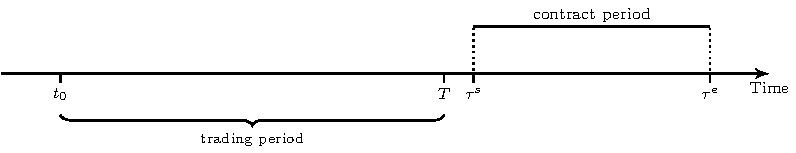
\includegraphics [scale = 0.9] {trading_period.pdf}
\caption{Trading and settlement periods for energy forward contract.}
\label{fig:trading_period}
\end{figure}

% changed "energy volume q" to "base load volume q" in text above 13.11.21 
% changed "hedged volume" to "transacted volume" below 13.11.21 and switched formulat for p_t
%The portfolio is protected from market risk via the hedge rate.
The price risk may be reduced by constructing a portfolio, consisting of the physical energy market exposure and derivatives contracts. The \textit{portfolio price} per energy unit $p_t$ is calculated as the weighted average of the value of the transacted volumes and the open volume evaluated mark-to-market
\begin{equation}
%p_t= \frac{p_t^h\times h_t q + f_t\times q (1-h_t)}{q} = f_t + (p^h_t - f_t)\times h_t
%p_t & = \bigg[f_0 h_0 q  + \sum_{i=1}^{t} f_i (h_i - h_{i-1}) q + f_t (1-h_t) q\bigg]/q \\
p_t = \frac{1}{q} \bigg(f_0 h_0 q  + \sum_{i=1}^{t} f_i (h_i - h_{i-1}) q + f_t (1-h_t) q\bigg) = f_0 h_0 + \sum_{i=1}^{t} f_i (h_i - h_{i-1}) + f_t (1-h_t) 
\end{equation}
where $h_t\in(0,1)$ is the hedge rate and $f_t$ the futures price at time $t$. In the simplest possible scenario, the risk can be managed by locking the entire volume in the forward market. This removes the price risk and the portfolio owner knows up front what to pay or receive when delivery of the energy takes place. On the downside, one might regret locking if the market develops in a favourable way. 

\subsection{Portfolio insurance strategies}

In the portfolio insurance approach, dynamic hedging strategies that allow buying and selling the hedging instrument are used to protect the portfolio, while seeking to benefit from advantageous market developments. Historically, the theory of portfolio insurance has focused on protection against downside risk in financial investment portfolios, see \citet{leland1976evolution} , \citet{perold1988dynamic} and \citet{Leland1980WhoSB}. Here, we apply the same principles to manage commodity price risk in the forward market. A consumer following a dynamic hedging program may control price risk by locking a share of future volume in the futures market, and increase (decrease) the share if the price increase (falls). A seller can implement similar strategies to maximise value of the energy portfolio. The size of the initial hedged share and how it is adjusted affects both the protective properties of the hedging scheme as well as its ability to exploit opportunities in the market. Trading activity needs to be carefully managed and harmonized with overall objectives and risk preferences. A variety of portfolio insurance strategies offer different approaches to this task. The allocation strategies presented below all aim to control $p_t$ and prevent breach of a pre-specified cap (or floor) price, $p^*$, under the hedge rate restriction $h_t\in(0,1)$.


The \textbf{Constant proportion portfolio insurance (CPPI)} strategy was introduced by \citet{perold1986constant} and  \citet{black1987simplifying} for management of investment portfolios with capital guarantees. When applied to an energy portfolio, it aims to insure the portfolio by protecting a target price, a cap (floor) value for the portfolio price. Prior to start of hedging, $p^*$ is set equal to the highest (lowest) acceptable portfolio price. This target price must be set higher than the first day's market price $f_0$ to implement cap protection, or lower for a floor protection model. The difference between the target price and the current portfolio price is termed the cushion. The key idea of CPPI is that the proportion of the volume exposed to the market should be calculated as a constant multiple $m$ of the cushion. The multiple is given by $m=\mu^{-1}$, where $\mu>0$ is a risk factor set to handle the maximum daily price change to be handled by the hedging model, which again affects strategy gearing. The unexposed proportion, the hedge rate,  is
\begin{equation}
h_t =
\begin{cases}
0 & \text{ if } \quad c_t > \mu\\
1-m c_t  & \text{ if } \quad \mu \geq c_t\geq 0 \\
1 & \text{ if } \quad c_t< 0
\end{cases}
\end{equation}
where $c_t=p^*-p_{t-1}$ for a short hedger, and  $c_t=p_{t-1}-p^*$ for the long hedger. 
%The risk factor determine the gearing of the energy portfolio, which again affects the strategy's vulnerability to gap risk.

In the \textbf{Dynamic proportion portfolio insurance (DPPI)} strategy, a decision rule similar to CPPI is applied, but the multiple $m_t$ is allowed to vary. Changing market conditions may require re-evaluation of the risk factor in the multiple. Methods such as Value-at-Risk or Expexted Shortfall, or even simple heuristics can be used for this purpose. For a further treatment of DPPI type strategies, the reader is referred to \citet{lee2008new} and \citet{chen2008dynamic}. In \CRANpkg{etrm} we also allow adjustments in the target price $p^*_t$, to catch opportunities to lower the capped value, or to increase the floor value. The hedge rate is determined similarly to CPPI, with
\begin{equation}
p^*_t =
\begin{cases}
min(\lambda p_{t-1},p^*_{t-1}) & \text{ short hedger }\\
\\
max(\lambda p_{t-1},p^*_{t-1}) & \text{ long hedger }
\end{cases}
\end{equation}
where $\lambda = \frac{p^*_o}{p_o}$ for a short hedger, and $\lambda = \frac{p_o}{p^*_o}$ for the long hedger.

\textbf{Option based portfolio insurance (OBPI)} was first introduced in \citet{leland1976evolution} as a means of providing insurance for investment portfolios. By combining an investment in a risky asset with a put option on the asset, the portfolio value is prevented from falling below the option strike price, K. A similar approach can be taken for the energy portfolio. As we are using futures contracts to manage the energy price risk, the Black-76 formula introduced in \citet{black1976pricing} is used to approximate the contingent claim premium. The price at time $t$ of the European call and put options with exercise date $T$ and strike price $K$, on a futures contract with delivery start $\tau^s \geq T$ is given by
\begin{eqnarray}
C(f_t, t, K, \sigma, r) &=& e^{-r (T-t)} [f_t N(d_1) - KN(d_2)]\\
P(f_t, t, K, \sigma, r) &=& e^{-r (T-t)} [KN(-d_2) - f_t N(-d_1)]
\end{eqnarray}
where $f_t$ is the futures price and $N$ is the cumulative distribution function of $N(0,1)$, where
\begin{eqnarray}
d_1 &=& \frac{\ln(f_t/K) + (\sigma^2/2)(T-t)}{\sigma\sqrt{(T-t)}}\\
d_2 &=& d_1 - \sigma\sqrt{(T-t)}
\end{eqnarray}
and $r$ is the risk free rate of interest, $\sigma$ the volatility of the underlying futures price and $(T-t)$ is the time to exercise date. The sensitivity in the option premiums with respect to changes in the underlying futures price is given by the call and put option deltas:
\begin{eqnarray}
\frac{\partial C}{\partial f} &=& e^{-r(T-t)}N(d_1)\\
\frac{\partial P}{\partial f} &=& e^{-r(T-t)}N(-d_1)
\end{eqnarray}
These are used to synthesise the option, by setting portfolio hedge rate $h_t\in(0,1)$ with the call (buyer) and put (seller) option deltas. By implementing this \textit{delta hedging} scheme, a cap (floor) for the portfolio price is set at the option strike price $K$, adjusted for the option premium/ replication costs. For a more detailed presentation of the underlying theory, the reader is referred to \citet{bjork2009arbitrage}.

\textbf{Step hedge portfolio insurance (SHPI)} is a simple and mechanical benchmark strategy that builds hedging positions gradually by transacting identical volumes each day through the trading period $(t_0, T)$, reaching a full hedge prior to the start of the settlement period. The hedge rate for a buyer at time $t$ is given by

\begin{equation}
h_t =
\begin{cases}
\frac{t}{T-t_0 +1} & \text{ if } \quad p_t < p^*\\
1  & \text{ if } \quad p_t \geq p^* \\
\end{cases}
\end{equation}
The hedges for a seller is entered mechanically in a similar manner as long as $ p_t > p^*$. In the event $p_t \leq p^*$ a full hedge $h_t = 1$ is implemented. By distributing the transacted volumes evenly across the trading period while monitoring the target, the strategy portfolio price will either be locked in at the target price, or end up equal to the average forward market price over $(t_0, T)$.

Finally, the \textbf{Stop loss portfolio insurance (SLPI)} is another simple benchmark, where no hedge positions are entered unless the target level is reached. For a buyer, this may be expressed as 

\begin{equation}
h_t =
\begin{cases}
0 & \text{ if } \quad p_t < p^*\\
1  & \text{ if } \quad p_t \geq p^* \\
\end{cases}
\end{equation}
For a seller, the logic is reversed with $h_t=0$ for $p_t > p^*$ and $h_t=1$ for $p_t \leq p^*$. In the event that the target level is reached, the portfolio is kept fully hedged until start of settlement. If this does not occur, the portfolio follows the forward market, leaving an option to lock in the price at contract expiration.

The strategies presented above all have strengths and weaknesses. CPPI, SHPI and SLPI are simple and intuitive, but can be vulnerable to so-called \textit{lock in}, the inability to improve portfolio price once the target level has been reached. This is also the case for DPPI. The OBPI does not suffer from this trait, but it relies on more assumptions regarding model parameters. In some scenarios, it will also generate more trading activity (costs), for example if the market fluctuate around the option strike price, $K$.  Finally, as the strategies must be implemented in discrete time, they will all be exposed to gap risk.

\subsection{The strategy classes with examples}
The portfolio insurance strategies in \CRANpkg{etrm} are implemented as S4 classes. Since they share many characteristics, they inherit most of their properties from a parent class,  \code{"GenericStrat"}. In fact, the implementation of the simple benchmark strategies SLPI and SHPI do not require any additional properties to be added to the parent. The remaining strategy classes have some additional model specific features, in accordance with the descriptions in previous section. This modular design offers flexibility, and new strategies for price risk management can easily be added to the package.

\begin{figure}[ht!]
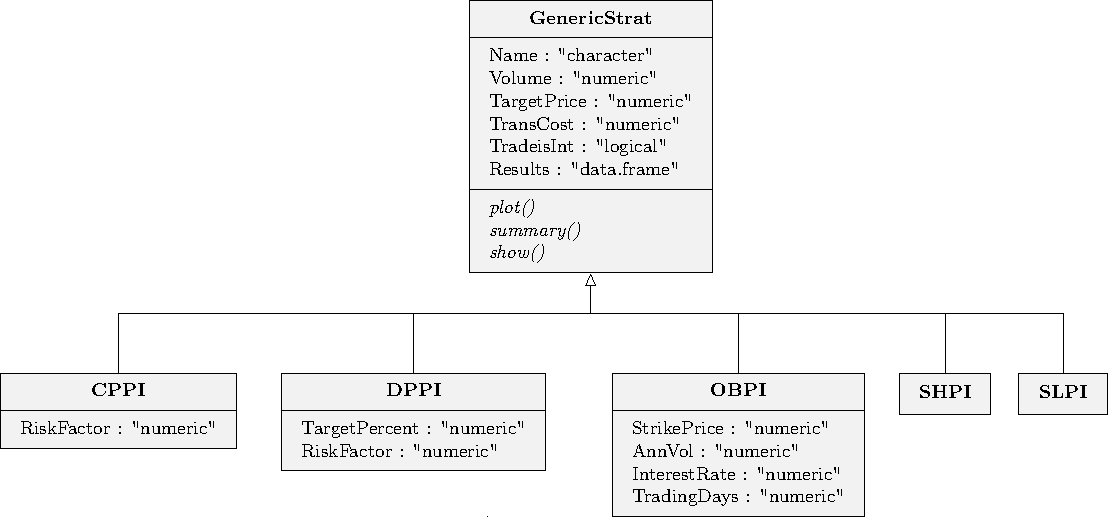
\includegraphics [scale = 0.7] {strategy_classes.pdf}
\caption{Attributes and methods for portfolio insurance strategy classes in the \CRANpkg{etrm} package.}
\label{fig:strategy_classes}
\end{figure}


Figure \ref{fig:strategy_classes} provide an overview of the class hierarchy, and a brief description is given in the following. In \code{"GenericStrat"}, the \code{"Name"} property is used to store a strategy identifier. Allowed character values are "CPPI", "DPPI", "OBPI", "SHPI" and "SLPI". The volume to be managed and the corresponding price cap (floor) can be found in \code{"Volume"} and \code{"TargetPrice"}, respectively. If a transaction cost has been included in the calculation of the portfolio price, this is to be found in \code{"TransCost"}. One may also set a restriction on transactions by requiring that the smallest volume available for trading is equal to 1 unit. This lot size limitation is stored as TRUE/FALSE in \code{"TradeisInt"}. The main output from a strategy calculation can be found in \code{"Results"}. This data frame keeps daily values for market prices, transactions, exposed volume, open volume, hedge rate, target price and portfolio price. 

The generic methods \code{plot()}, \code{summary()} and \code{show()} are implemented in \code{"GenericStrat"} and inherited by the strategy classes. The \code{plot()} method returns a chart based on \code{"Results"}, with daily values for portfolio, market and target prices and portfolio hedge rate. The \code{summary()} method returns a list with five elements; a description string, portfolio volume, target price, calculated churn rate and a data frame with summary statistics for the trading period. Finally, the \code{show()} method returns the \code{"Results"} data frame.

\begin{table}[ht!]
\centering
\begin{tabular}{lll}
\toprule
\textbf{Argument} & \textbf{Description} & \textbf{Default value} \\
\midrule
\code{q} & Numeric volume & none \\
\code{tdate}  & Date vector with trading days & none \\
\code{f} & Numeric price vector & none \\
\code{tcost} & Numeric transaction cost & 0 \\
\code{int} & Logical lot size integer restriction & TRUE \\
\bottomrule
\end{tabular}
\caption{Arguments shared by the portfolio insurance strategy functions.}
\label{shared_arguments}
\end{table}

The strategy constructor functions \code{cppi()}, \code{dppi()}, \code{obpi()}, \code{shpi()} and \code{slpi()} share five of the arguments, see Table \ref{shared_arguments}. Each strategy require some additional arguments to implement the models presented in previous section. All of these inputs are of \code{"numeric"} data type. They are summarised in Table \ref{strategy_arguments}.

\begin{table}[ht!]
\centering
\begin{tabular}{llll}
\toprule
%\multicolumn{4}{c}{Team sheet} \\
%\hline
\textbf{Function} & \textbf{Argument} &  \textbf{Description} & \textbf{Default value} \\ \midrule
\multirow{2}{*}{\code{cppi()}}
 & \code{tper} & Target price factor & none\\
 & \code{rper} & Risk factor percentage & none \\ 
 \hline
\multirow{2}{*}{\code{dppi()}}
 & \code{tper} & Target price factor & none\\
 & \code{rper}  & Risk factor percentage & none\\ 
 \hline
\multirow{4}{*}{\code{obpi()}}
 & \code{k} & Option strike price & $k=f_0$\\
 & \code{vol} & Annualized volatility &  none\\
 & \code{r} & Interest rate & 0 \\
 & \code{tdays} & Trading days per year & 250\\ 
  & \code{daysleft} & Days left to expiry & none\\ 
  \hline
  \multirow{2}{*}{\code{shpi()}}
 & \code{tper} & Target price factor & none\\
 & \code{daysleft} & Days left to expiry & none\\ 
 \hline
   \multirow{1}{*}{\code{slpi()}}
 & \code{tper} & Target price factor & none\\
 \bottomrule
\end{tabular}
\caption{Model specific arguments for the portfolio insurance strategy functions.}
\label{strategy_arguments}
\end{table}


To illustrate further, we proceed with an example. Consider a European consumer of electricity procuring 30 MW to be delivered in 2006. The CAL-06 baseload power future from the synthetic \CRANpkg{etrm} \code{"powcal"} data set is used as hedging instrument. Trading is started 500 days prior to the contract expiry, approximately a horizon of 2 years. For the \code{"OBPI"} strategy presented below, the target price is calculated as an expected price cap given by the option premium-adjusted strike price selected for the delta hedging scheme within a standard Black-76 option pricing framework. The default \code{obpi()} strike price is set at-the-money, in this case at 26.82 EUR/MWh. The expected target price illustrated with the horizontal dotted line in Figure \ref{fig:cal06_obpi_long} is calculated to be 29.84 EUR/MWh. The \code{"OBPI"} delta hedging scheme dictate an initial hedge rate of 57 percent, and the consumer enters a 17 MW position in CAL-06 on the first day of trading.

As time progresses and the market price changes, the \code{obpi()} function adjust the required hedge rate in order to replicate the call option on the CAL-06 contract. Hedge rate is gradually built up as the market increase from the second quarter of 2004, followed by a reduction after the sharp price drop starting late in the same year. Eventually, the volume is fully hedged due to the strong upwards price trend in 2005. The CAL-06 contract closes at 37.81 EUR/MWh on the expiry date, while the consumer has a hedge of 30 MW and a portfolio price of 29.29 EUR/MWh. The calculated price of the option to be synthesized (and the delta hedges) will depend on the Black-76 model parameters. In this example the risk free rate of interest is set to $r=0$ and annualized volatility $\sigma$ is assumed to be 20 percent. The following code will implement the strategy and create the plot in Figure \ref{fig:cal06_obpi_long}:

%dat06 <- data.frame(Date = tail(powcal\$Date[!is.na(powcal\$Date)], 500)\hspace{3cm} CAL06 = tail(powcal\$`CAL-06`[!is.na(powcal\$`CAL-06`)], 500))

\begin{example*}
# data frame with final 500 trading days for CAL-06 contract
dat06 <- tail(na.omit(powcal[, c(1,2)]), 500)

# instance of the OBPI class
cal06_obpi_b <- obpi(q = 30,
\hspace{3cm} tdate = dat06\$Date,
\hspace{3cm} f = dat06\$`CAL-06`,
\hspace{3cm} k = dat06\$`CAL-06`[1],
\hspace{3cm} vol = 0.2,
\hspace{3cm} r = 0,
\hspace{3cm} tdays = 250,
\hspace{3cm} daysleft = 500,
\hspace{3cm} tcost = 0,
\hspace{3cm} int = TRUE)

# the generic plot() method
plot(cal06_obpi_b, title = "", legend = "right", ylab.1 = "EUR/MWh")
\end{example*}

\begin{figure}[ht!]
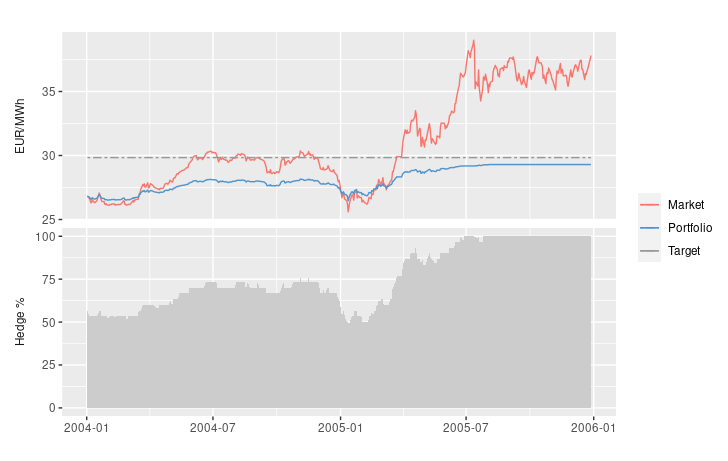
\includegraphics [scale = 0.7] {cal06_obpi_long.png}
\caption{Option based portfolio insurance (OBPI) strategy for buyer CAL-06. Daily observations for prices (top panel) and hedge rate (bottom panel). As the market price continue to rise, the hedge rate is increased and the portfolio price is locked below the target price level.}
\label{fig:cal06_obpi_long}
\end{figure}

An aggregated view of the trading activity over the 2 year period  and final results can be retrieved by running the \code{summary()} method on the object created above:\\

\begin{example*}
> summary(cal06_obpi_b)
\$Description
[1] "Hedging strategy of type OBPI and length 500"

\$Volume
[1] 30

\$Target
[1] 29.83626

\$ChurnRate
[1] 4.333333


\$Stats
      Market Trade Exposed Position     Hedge   Target Portfolio
First  26.82    17      13       17 0.5666667 29.83626  26.82000
Max    39.01    17      17       30 1.0000000 29.83626  29.29433
Min    25.60    -3       0       13 0.4333333 29.83626  26.46833
Last   37.81     0       0       30 1.0000000 29.83626  29.29433
\end{example*}

\noindent We note from the \code{"ChurnRate"} that the underlying 30 MW volume had to be traded 4.33 times in order to synthesize the call option and achieve the results summarised in \code{"Stats"}. By also considering the trading costs in the calculations, the user can get valuable inputs when considering alternatives, such as simply buying the option in the market. However, such contract may not always be available.   

Finally, the \code{show()} method provide details regarding daily values for market price, transactions, exposed volume, futures contract position, hedge rate, the target price and the calculated portfolio price:

\begin{example*}
> head(show(cal06_obpi_b))
        Date Market Trade Exposed Position     Hedge   Target Portfolio
1 2004-01-02  26.82    17      13       17 0.5666667 29.83626  26.82000
2 2004-01-05  26.63    -1      14       16 0.5333333 29.83626  26.73767
3 2004-01-07  26.31     0      14       16 0.5333333 29.83626  26.58833
4 2004-01-08  26.31     0      14       16 0.5333333 29.83626  26.58833
5 2004-01-09  26.54     0      14       16 0.5333333 29.83626  26.69567
6 2004-01-12  26.32     0      14       16 0.5333333 29.83626  26.59300
\end{example*}


For the sake of comparison, the OBPI strategy for CAL-06 from a sellers point of view can be implemented with similar assumptions by setting the volume to $q = -30$. Using the default at-the-money strike price, the seller calculates an expected target floor to protect at 23.80 EUR/MWh and an initial hedge rate of 43 percent. As the market starts to rise, the hedge is reduced. The seller increases the hedge in late 2004 to dampen the effect from the market drop, and finally exits the forward market positions as the price increases during 2005. The portfolio price follows the market upwards with a premium for the put option replication,  as expected for an insurance scheme. The CAL-06 contract closes at 37.81 EUR/MWh, and the seller has a portfolio price of 35.34 EUR/MWh, which may be locked in on the final trading day.

\begin{figure}[ht!]
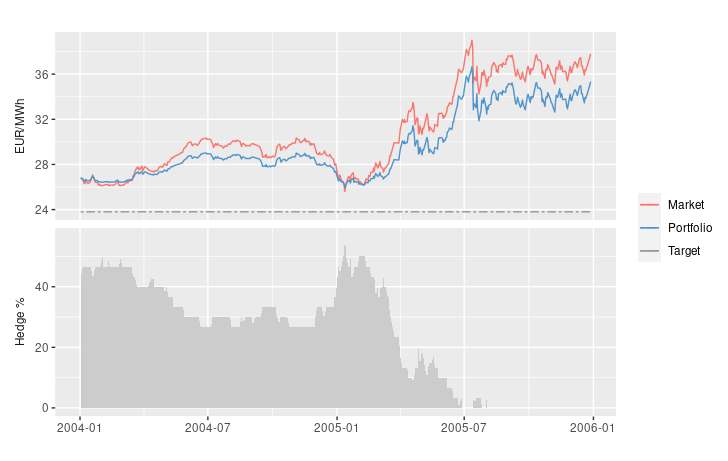
\includegraphics [scale = 0.7] {cal06_obpi_short.png}
\caption{Option based portfolio insurance (OBPI) strategy for seller CAL-06. Daily observations for prices (top panel) and hedge rate (bottom panel). The hedge rate is lowered in the upwards trending market, and the portfolio price continue to increase.}
\label{fig:cal06_obpi_short}
\end{figure}

\newpage

\begin{example*}
# instance of the OBPI class
cal06_obpi_s <- obpi(q = - 30,
\hspace{3cm} tdate = dat06\$Date,
\hspace{3cm} f = dat06\$`CAL-06`,
\hspace{3cm} k = dat06\$`CAL-06`[1],
\hspace{3cm} vol = 0.2,
\hspace{3cm} r = 0,
\hspace{3cm} tdays = 250,
\hspace{3cm} daysleft = 500,
\hspace{3cm} tcost = 0,
\hspace{3cm} int = TRUE)

# the generic plot() method
plot(cal06_obpi_s, title = "", legend = "right", ylab.1 = "EUR/MWh")
\end{example*}




\begin{example*}
> summary(cal06_obpi_s)
\$Description
[1] "Hedging strategy of type OBPI and length 500"

\$Volume
[1] -30

\$Target
[1] 23.80374

\$ChurnRate
[1] 4.2

\$Stats
      Market Trade Exposed Position     Hedge   Target Portfolio
First  26.82   -13     -17      -13 0.4333333 23.80374  26.82000
Max    39.01     2     -13        0 0.5666667 23.80374  36.64867
Min    25.60   -13     -30      -17 0.0000000 23.80374  25.95167
Last   37.81     0     -30        0 0.0000000 23.80374  35.33567
\end{example*}




In the examples above, we have implicitly assumed that both the consumer and the seller have a flat volume corresponding to 30 MW over the entire year which can be covered by a base load contract such as the CAL-06. In practice, this is typically not the case. Industrial energy consumers will have consumption profiles determined by the activity level in their production facilities, and often face seasonal shifts due to variation in demand, or holidays. Weather also play a large role, both for consumers and producers such as hydroelectric plants. In order to hedge the predicted volume more precisely, some of the other contract types presented in Table \ref{powfutures130513} will need to be included in the portfolio. Market players will "roll forward" and start trading contracts covering shorter periods such as quarters, months and weeks, as they become available. The mandate for the energy portfolio will typically be broken down into smaller time intervals with expected volume and required hedge levels. All strategies presented here may be used to make decisions for several years and their sub periods, and the market value of a specific volume prognosis and corresponding futures positions can be evaluated using the forward curve discussed in previous sections.

In order to maintain focus on the strategies themselves, we continue with the baseload example with 30 MW. In Figure \ref{fig:buyer_strat} we plot results for the remaining four strategies for the consumer hedging with CAL-06. The benchmark strategies \code{"SHPI"}, and \code{"SLPI"} follow simple, mechanical patterns. The \code{"SHPI"} builds a full hedge gradually over the trading period, ending at either the average forward market price for the period, or the target price. This approach will always ensure a full hedge at expiry, without intervention. The \code{"SLPI"} does not take any positions unless the target is reached, ending either at the target level, or leaving an option to close at the contract expiry price. As the CAL-06 increase significantly during 2005, both end up at the target level.

\begin{figure}[!htb]
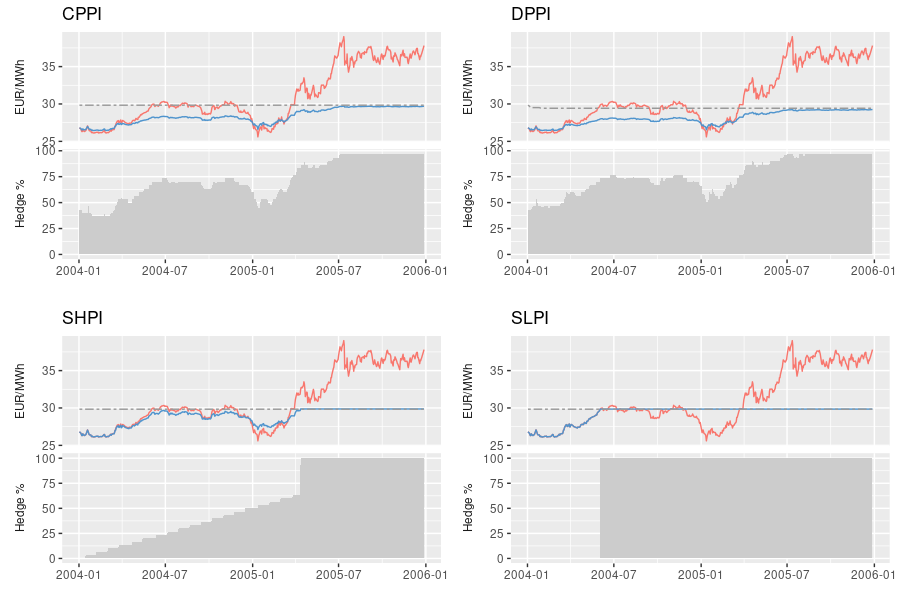
\includegraphics [scale = 0.58] {buyer_strat.png}
\caption{Achieved results for the strategies CPPI, DPPI, SHPI and SLPI for buyer CAL-06. Daily observations for prices (top panels) and hedge rate (bottom panels).}
\label{fig:buyer_strat}
\end{figure}

The \code{"CPPI"}, and \code{"DPPI"} strategies are more dynamic and adjust hedge rate according to market developments and the model parameters. As the \code{"DPPI"} implements a dynamic risk factor, $\mu_t$, the strategies are geared differently. In this example, the \code{"DPPI"} successfully adjusts the target price downward on one of the first trading days, and achieves a lower portfolio price on last trading day.

A similar overview from a seller's perspective is provided in Figure \ref{fig:seller_strat}. As the market trends upwards during the hedging period, none of the strategies end up at the initial target price. The \code{"SHPI"} builds the hedge positions in a step-wise manner, ending up with a portfolio price equal to the average futures market price for the period. The \code{"SLPI"} does not enter any positions, leaving an option to lock in market price at expiry. Finally, we can also here see some differences between \code{"CPPI"}, and \code{"DPPI"}. This is due to the dissimilar gearing of the portfolios, but also because of the rather frequent adjustments of the target price by \code{"DPPI"}. In order to protect the higher targets, hedge rate must be increased and \code{"DPPI"} falls behind \code{"CPPI"} and ends up at a lower portfolio price for the seller.


\begin{figure}[!htb]
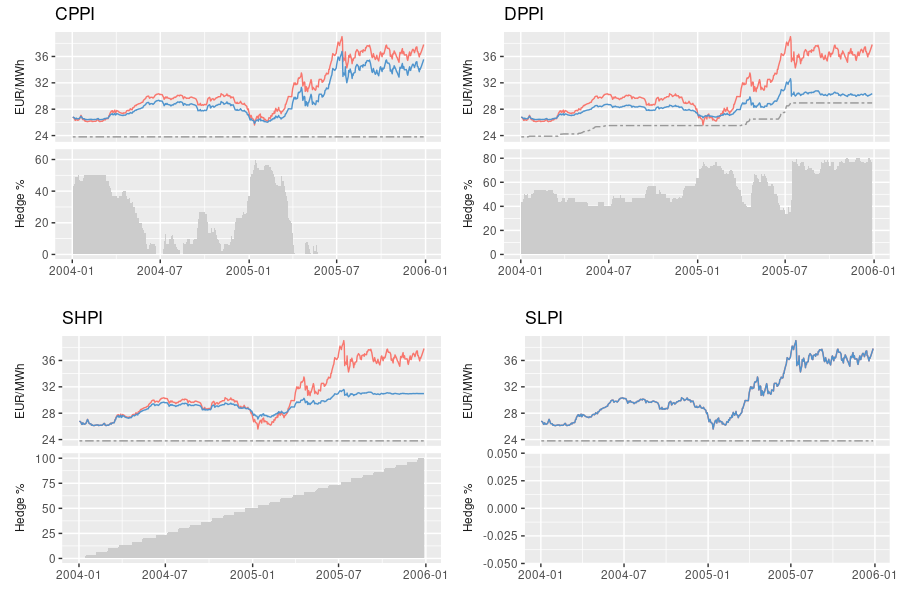
\includegraphics [scale = 0.58] {seller_strat.png}
\caption{Achieved results for the strategies CPPI, DPPI, SHPI and SLPI for seller CAL-06. Daily observations for prices (top panels) and hedge rate (bottom panels).}
%\caption{Achieved insurance strategy hedge rates and portfolio prices for seller CAL-06.}
\label{fig:seller_strat}
\end{figure}

\newpage

\CRANpkg{etrm} can also be used in conjunction with other R packages to evaluate risks related to energy procurement. Metrics such as \textit{Value-at-Risk} and \textit{Expected Shortfall} can for example be calculated using the \CRANpkg{PerformanceAnalytics} package. We will proceed with a simple, illustrative example. Consider the OBPI portfolios \code{"cal06\_obpi\_b"} and \code{"cal06\_obpi\_s"} in the code example above. If we need to calculate risk measures at a specific point in time, say at day $350$ in the trading period, we can execute the following code:


\begin{example*}
library(PerformanceAnalytics)

# CAL-06 returns prior to t=350
ret_06 <- head(diff(log(show(cal06_obpi_b)\$Market)), 349)

# portfolio status at t=350
pdat <- rbind(
  Buyer =show(cal06_obpi_b)[350,],
  Seller =show(cal06_obpi_s)[350,]
)
  
# add risk measures to pdat
pdat <-cbind(pdat, 
      VaR = abs(rep(VaR(ret_06, p=.95, method="historical"), 2)*pdat$Market*pdat$Exposed*8760),
      ES = abs(rep(ES(ret_06, p=.95, method="historical"), 2)*pdat$Market*pdat$Exposed*8760))
\end{example*}

The calculation above evaluate market risk related to the unhedged volume (exposed MW $\times 8760$ hours in the year 2006) at current market prices under the (simplistic) assumption of symmetry in the returns distribution. The portfolio status, including risk metrics is

\begin{example*}
> pdat[c(-1, -3)]
       Market Exposed Position Hedge   Target Portfolio VaR         ES
Buyer   32.54       3       27   0.9    29.84  28.98     10671.55    18237.06
Seller  32.54     -27       -3   0.1    23.81  30.38    96043.94    164133.52
\end{example*}


\section{Overview of the etrm package}
Package \CRANpkg{etrm} offers an open source implementation of core functionalities of an ETRM system:

\begin{itemize}
  \item Construction of forward curves
  \item Strategies for price risk management
\end{itemize}
Functions included in the package are listed in Table \ref{function_overview}.

\begin{table}[ht!]
\centering
\begin{tabular}{lll}
\toprule
\textbf{Function} & \textbf{Description}  \\
\midrule
\code{msfc()} & Maximum Smoothness Forward Curve  \\
\code{cppi()}  & Constant Proportion Portfolio Insurance \\
\code{dppi()} & Dynamic Proportion Portfolio Insurance\\
\code{obpi()} & Option Based Portfolio Insurance \\
\code{shpi()} & Step Hedge Portfolio Insurance \\
\code{slpi()} & Stop Loss Portfolio Insurance \\
\bottomrule
\end{tabular}
\caption{Overview of \CRANpkg{etrm} package functions}
\label{function_overview}
\end{table}

All functions act as constructors for their corresponding S4 classes, as described in further detail in previous sections. The classes all have generic methods \code{plot()}, \code{summary()} and \code{show()}. Unit tests covering all functions in \CRANpkg{etrm} have been implemented using the \CRANpkg{testthat} framework introduced in \citet{wickham2011testthat}. 

Three synthetic data sets are included in the package, see Table \ref{data_overview}. The \code{"powfutures130513"} and \code{"powpriors130513"} data may be used to create forward curves with the \code{msfc()} function for the trading date 2013-05-13. The portfolio insurance strategies may be tested on the \code{"powcal"} data set, which contains historical prices for 11 base load power futures.
\\
\begin{table}[ht!]
\centering
\begin{tabular}{lll}
\toprule
\textbf{Data set} & \textbf{Description}  \\
\midrule
\code{powfutures130513} & Synthetic data for a set of electricity base load futures \\
& quoted at 2013-05-13. Closing prices for contracts with\\
 & weekly, monthly, quarterly and yearly settlement periods \\
\\
\code{powpriors130513} & Two simple priors for forward market price curve\\
& Daily values for calculation to be used with powfutures130513 \\
\\
\code{powcal} & Synthetic data set with daily closing prices for 11 electricity \\
& base load futures with yearly settlement periods for 2006-2016 \\
\bottomrule
\end{tabular}
\caption{Overview of \CRANpkg{etrm} package data sets}
\label{data_overview}
\end{table}


\section{Summary and suggestions for future work}

This paper introduces \CRANpkg{etrm}, an R package for energy market risk management. The package contains tools previously not available in the R ecosystem, such as the \code{msfc()} function for building a forward curve for energy commodities with flow delivery contracts and strong seasonality. The forward curve is a key decision making tool with many uses, such as pricing non-standard supply agreements, investment decisions and risk management. \CRANpkg{etrm} also provides implementations of portfolio insurance strategies for handling price risk, suitable for both long and short hedgers. The functions can be used for back testing strategies on historical futures price data, risk and strategy evaluations, and as decision support tools for trade execution.

The \CRANpkg{etrm} package may be developed further by incorporating new elements. First, the forward curve calculation may be done on an hourly level. The bid-ask spread can be used as price constraint for the optimization, as an extension of the current solution based on closing prices. Competing forward curve calculation methods can also be added to the package, and new asset allocation strategies for price risk management could be included. 

A further extension of \CRANpkg{etrm} functionality can be to implement a \code{"PORTFOLIO"} class, consisting of a daily volume prognosis covering the full management horizon, supplemented with authorized volumes per (sub)period and hedging strategy objects implemented in accordance with these authorizations. The portfolio object could contain multiple strategy objects for contracts such as "year", "quarter", "month" and "week", depending on the shape of the volume prognosis. This construction can be priced using the forward curve, and portfolio wide risk measures could be calculated via Monte Carlo simulations on the curve.


\section{Acknowledgments}
We thank the editor and two anonymous reviewers for their constructive comments, which helped us to improve the manuscript. This work has been supported by The Norwegian Research Council via the industrial Ph.D. scheme. The author also wish to thank Montel AS and former colleagues in Kinect Energy Markets AS for interesting discussions and helpful comments.

\bibliography{sleire.bib}

\address{Anders D. Sleire\\
  Department of Mathematics\\
  University of Bergen\\
  P.O.Box 7803\\
  N-5020 Bergen\\
  Norway\\}
\email{Anders.Sleire@uib.no}
